\section{Methodology}
\label{s:method}

\subsection{Data Sources}
\label{ss:data}

\paragraph{choosealicense.com.} The repository behind choosealicense.com~\cite{choosealicense} contains 47 license files, each with a YAML header and the full license text. We keep the SPDX identifier, title, description, the three label lists, and the text, and drop website-only fields (installation instructions, example projects, display flags). The label vocabulary has 5 permissions (commercial use, modifications, distribution, private use, patent use), 8 conditions (include copyright, include copyright in source, document changes, disclose source, same license, same license for files, same license for libraries, network use is distribution), and 4 limitations (liability, warranty, trademark use, patent use). These labels are the facts from which all our ground truth is computed.

\paragraph{SPDX license list.} From the SPDX list (v3.29.0, 740 identifiers)~\cite{spdx} we keep each identifier and its OSI-approval flag, used to scope the catalogue and to normalise dependency licenses.

\paragraph{Software Heritage license dataset.} This dataset~\cite{zacchiroli2022dataset} describes 6.5 million deduplicated license files from public software origins. We use five metadata tables (file names and identifiers, file information, ScanCode license detections, first appearance and popularity, example origin) and the published 20{,}000-file random text sample; we do not download the 14\,GB full-text archive. The sample is joined to the five tables on two keys (SHA1 content hash and Software Heritage identifier), producing a 20{,}000-row table with 16 columns. It is used for exploratory analysis and to measure scope coverage, not as ground truth.

\paragraph{Package registries.} At run time, dependency licenses are read from PyPI (\texttt{license\_expression}, \texttt{license}, then trove classifiers) and npm (\texttt{license}), and normalised to SPDX identifiers with exact matching and 41 common spellings. Development-only dependencies are ignored because they are not shipped.

\subsection{Scope and Preprocessing}
\label{ss:prep}

We remove licenses not intended for software (8: media, documentation, data, fonts, and hardware licenses) and licenses not approved by the OSI (5), leaving \textbf{34 in-scope licenses}. A language check (share of common French words per paragraph) identifies CeCILL-2.1 as French-only; it remains recommendable, but its claims cannot be verified by the English-only verifier. Each license is classed as permissive (21), weak copyleft (4), or strong copyleft (9) directly from its labels.

\paragraph{Clause segmentation.} The verifier accepts at most 512 tokens, while GPL-3.0 alone is about 35{,}000 characters; claims must also be checked against the one passage that supports them, and users need a specific passage as evidence. We therefore split each license into clauses: split at blank lines, drop non-English paragraphs, merge short headings into the following paragraph, and attach a paragraph ending in a colon (a lead-in) to each list item below it, so that no clause stops at ``\ldots to do the following:'' (Figure~\ref{fig:clauses}). This yields \textbf{812 clauses} from 33 English licenses (median 329 characters; all within the verifier's input limit).

\begin{figure}[tb]
    \centering
    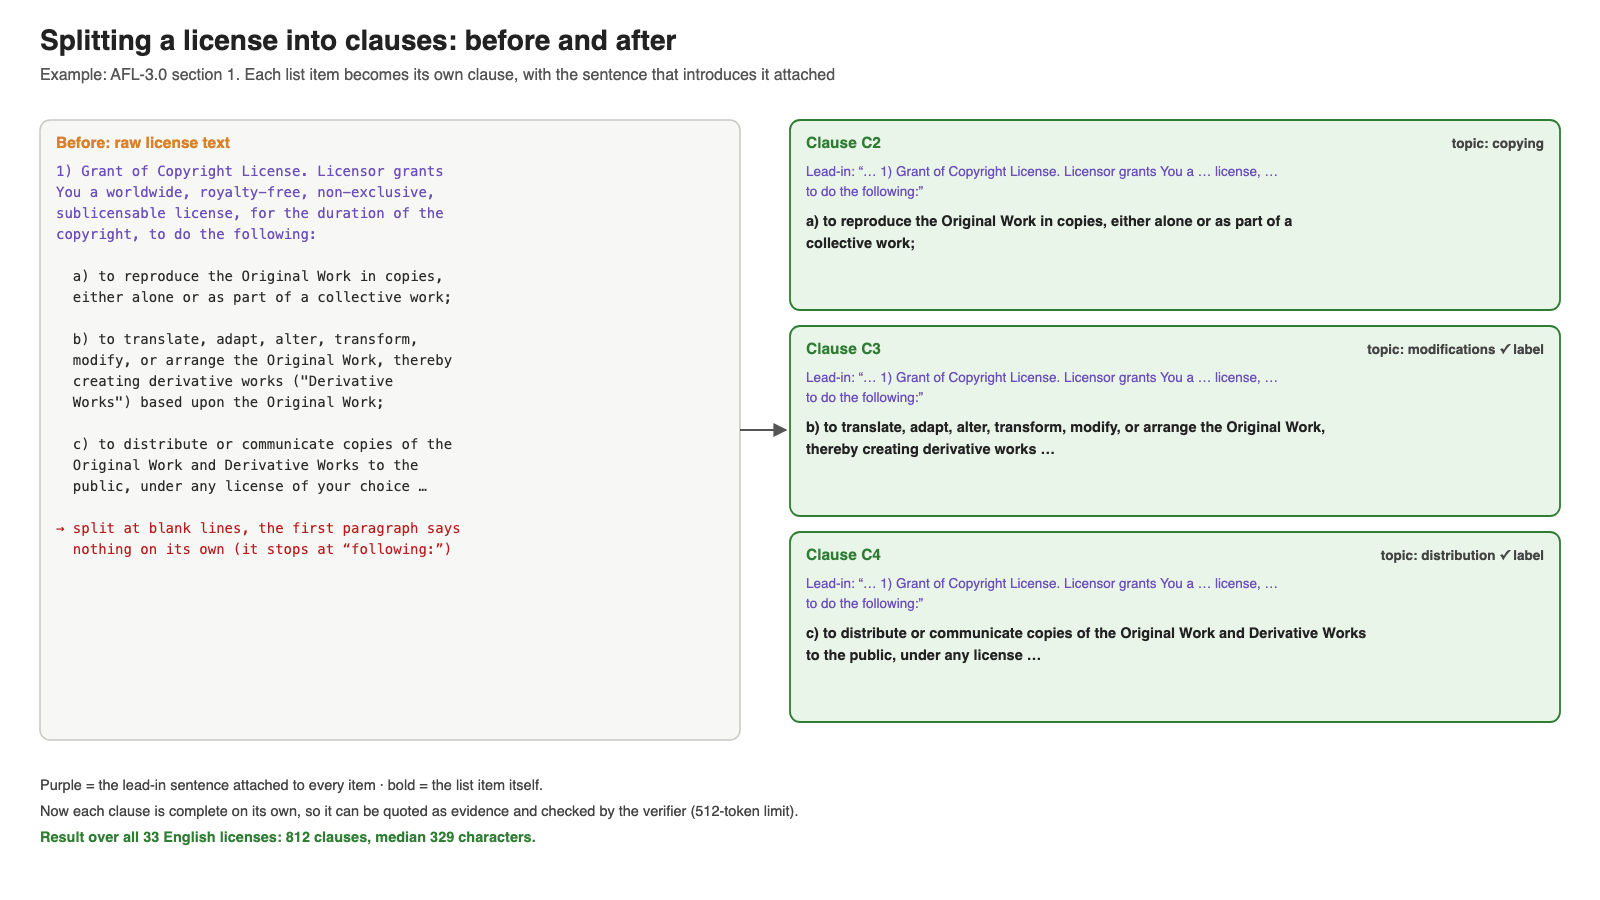
\includegraphics[width=\columnwidth]{25_clause_split.png}
    \caption{Clause segmentation on AFL-3.0: each list item becomes a clause with its lead-in sentence attached.}
    \label{fig:clauses}
\end{figure}

\paragraph{Finding the clause for a label.} For each of 16 labels we define a precise anchor pattern (e.g., ``Limitation of Liability'', ``Grant of Patent License'') and a broader keyword pattern. Clauses are ranked by anchor matches, then keyword matches, then position. We checked the selections by hand on MIT, BSD, Apache-2.0, GPL-3.0, and MPL-2.0. The same procedure selects evidence clauses for Stage~2 at run time.

\subsection{Ground Truth for RQ1: Profiles and Descriptions}
\label{ss:gt1}

No public dataset pairs developer requests with known correct licenses, so we construct one in which the answers are computed rather than judged.

\paragraph{Requirement profiles.} From the 17 labels we keep those that differ between in-scope licenses and that a developer would state as a need, giving six requirements: share changes (none, file/library level, whole work), network use (must trigger sharing, must not), patent grant, trademark protection, no attribution required, and no obligation to document changes. Labels held by every license (e.g., commercial use, warranty disclaimer) or by none are excluded because they cannot distinguish licenses. Allowing ``don't care'' for each requirement gives $4 \times 3 \times 2 \times 2 \times 2 \times 2 = 192$ combinations, or 191 excluding the empty request. For each combination, the \emph{answer key} is the set of in-scope licenses whose labels satisfy every requirement. 114 combinations have no satisfying license and are discarded, leaving \textbf{77 profiles} with 1 to 29 correct licenses each (median 3).

\paragraph{Natural-language descriptions.} Real developers describe projects in their own words rather than as requirement lists, and with structured requirements a simple label lookup, the same one that builds the answer key, would make an LLM unnecessary. We therefore test the recommender on natural-language descriptions. Qwen3.8-27B writes about three first-person descriptions per profile, each from a different persona and project type and never naming a license; persona variety tests whether the system understands meaning rather than one phrasing. gpt-oss-20b then reads each description \emph{without} the profile and lists the requirements it can identify; a description is kept only if they match the profile exactly. Of 235 descriptions written, \textbf{190} (81\%) pass, covering 70 of the 77 profiles. The writer produced 122 distinct persona labels, most often ``startup founder'' (29) and ``university researcher'' (25).

\subsection{Ground Truth for RQ2: Clause--Claim Pairs}
\label{ss:gt2}

For each English license and each label it carries, we take the clause selected for that label and build three pairs from 16 claim templates (one true and one negated sentence per label; private use is excluded because no license states it in a single clause): the true claim (\emph{entailment}), the negated claim (\emph{contradiction}), and a true claim about another label whose keywords do not appear in the clause (\emph{neutral}). Of 266 license--label combinations, 23 have no matching clause (mostly commercial use, as licenses such as BSD never mention selling), leaving 243 and therefore \textbf{729 pairs} (243 per label) built on 173 distinct clauses. The claims and labels are written by templates, not by any model; the NLI model only predicts labels for evaluation.

\paragraph{Human validation.} Because the labels are automatic, two annotators checked a stratified random sample of 150 pairs (50 per label): the first author, and a software engineer with experience working with open-source licenses who is now a software engineering researcher. Each labelled 75 pairs, judging only from the given clause. Disagreements with the automatic labels (22) were settled by the team; 3 remained ambiguous and were excluded, leaving \textbf{146 labelled pairs}. A later fix to clause segmentation changed 23 sampled pairs, which were relabelled. To measure inter-annotator agreement, each annotator also labelled 20 of the other's pairs.

\subsection{Evaluation Protocol and Metrics}
\label{ss:metrics}

\paragraph{RQ1.} Stage~1 (gpt-oss-120b) receives only the description text and the catalogue. For each description we compute Hit@1 (the first recommendation is in the answer key), Hit@3 (at least one of the three is), and Precision@3 (the share of the three that are), and for each requirement the share of recommendations that violate it. Results are grouped by the size of the answer key (1--3, 4--10, more than 10 correct licenses) as a measure of request specificity. Groq's free tier limits gpt-oss-120b to 200{,}000 tokens per day, so we evaluated one description per profile first and stopped at \textbf{104 descriptions covering all 70 profiles}.

\paragraph{RQ2.} DeBERTa-v3-large and RoBERTa-large-MNLI are run on all 729 pairs (premise = clause, hypothesis = claim). We report accuracy, per-class precision, recall, and F1, and macro-F1, against the automatic labels and against the 146 human labels. The key metric is \emph{entailment precision}: how often a \emph{verified} status is correct. Agreement is measured with Cohen's $\kappa$~\cite{cohen1960kappa}.

\paragraph{RQ3.} For complete pipeline runs we measure the share of quotes found verbatim in their cited clause and the distribution of verified, unverified, and contradicted claims. In Phase~1 this is limited to two end-to-end runs; the comparison with an unverified (LLM-only) baseline is planned for Phase~2.
